\phantomsection
\subsubsection*{Օգտագործողի կողմից կառավարվող տվյալների վերլուծության հարցումներ}\label{subsubsec:taintAnalisys}
\addcontentsline{toc}{subsubsection}{Օգտագործողի կողմից կառավարվող տվյալների վերլուծության հարցումներ}
Ծրագրային կոդի հատկությունների հարցումների համակարգի կարևոր բաղկացուցիչն է օգտագործողի կողմից կառավարվող տվյալների վերլուծության հարցումները:
Այս հարցումների նպատակն է օգտագործողներին հնարավորություն տալ վերլուծել, թե ինչպես են իրենց ծրագրի մեջ օգտագործվում
օգտագործողի կողմից մուտքագրված տվյալները:
Այս հարցումների միջոցով օգտագործողները կկարողանան ստանալ տեղեկություններ ծրագրի կատարման ընթացքում օգտագործողի կողմից
կառավարվող տվյալների հոսքի մասին, իմանալ, թե ծրագրի ինչ հատվածներում են այդ տվյալները օգտագործվում, ինչպիսի փոփոխականների
հետ են փոխազդում, ինչպես նաև կկարողանան արձանագրել սխալներ կամ անվտանգության խոցելիություններ, որոնք կարող են առաջանալ օգտագործողի
մուտքագրած տվյալների հետ փոխազդեցության արդյունքում:

\begin{figure}[h]
    \centering
    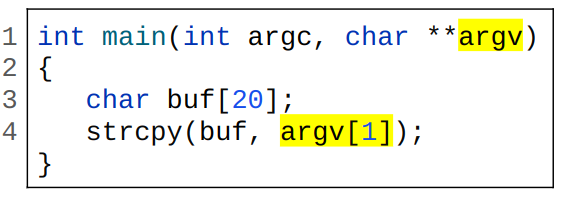
\includegraphics[width=0.4\textwidth]{pic16a}
    \caption{Բուֆերի գերբեռնում պարունակող աղբյուր կոդ}
    \label{fig:figure16a}
\end{figure}

Նկար \ref{fig:figure16a}-ում ներկայացված է բուֆերի գերբեռնում պարունակող աղբյուր, 4-րդ տողի strcpy ֆունկցիայի երկրորդ արգումենտը (argv[1])
կառավարվում է օգտագործողի կողմից, և հնարավոր է հանգեցնի բուֆերի գերբեռնման։
Նկար \ref{fig:figure16b}-ում նկարագրված հարցումների միջոցով օգտագործողը գտնում է strcpy ֆունկցիայի երկրորդ արգումենտի վրա ազդող, ագտագործողի կողմից
կառավարվող հրահանգները (tainted\_paths), և եթե այդ բազմությունը դատարկ չէ, տեղեկացնում է, որ առկա է բուֆերի գերբեռնում։

\begin{figure}[h]
    \centering
    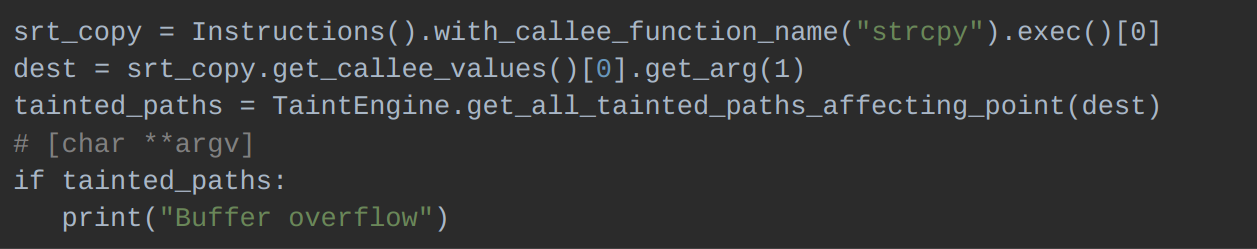
\includegraphics[width=0.9\textwidth]{pic16b}
    \caption{Օգտագործողի կողմից կառավարվող տվյալների վերլուծության հարցումների օրինակ}
    \label{fig:figure16b}
\end{figure}
